\section*{Analiza porównawcza spójności wyjaśnień}

W tej sekcji przeprowadzono ocenę spójności wyjaśnień generowanych przez różne metody XAI: LIME, SHAP i GradCAM.
Celem analizy było zrozumienie, jak bardzo wyjaśnienia nakładają się na siebie oraz jak różne techniki identyfikują istotne cechy obrazu.
Spójność wyjaśnień oceniono za pomocą współczynnika Intersection over Union (IoU) między obszarami wyjaśnień generowanych przez różne metody.

\begin{figure}[h]
	\centering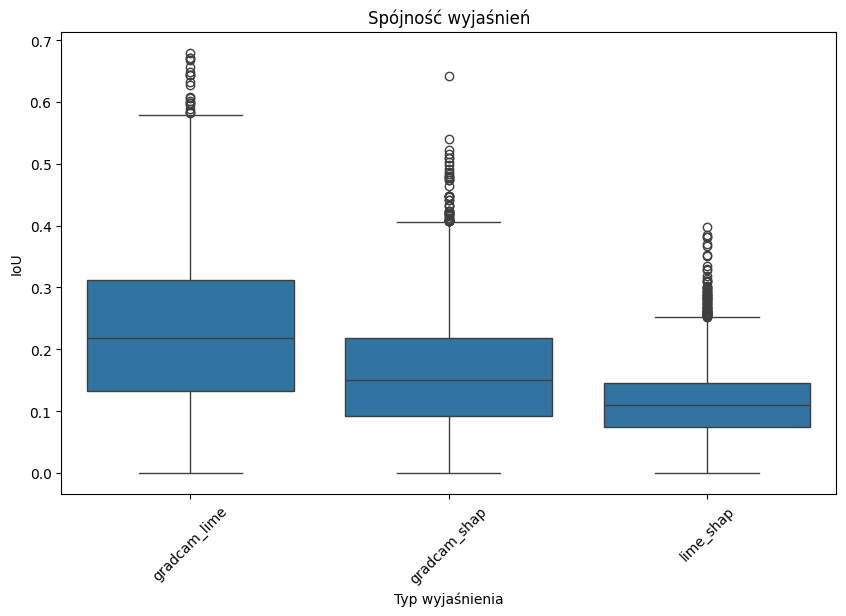
\includegraphics[width=.9\textwidth]{img/base_coherence}
	\caption{Spójność wyjaśnień}  \label{rys:base_coherence}
\end{figure}

\begin{table}[h]
	\centering
	\begin{tabular}{|c|c|}
		\hline
		\textbf{Metody XAI}     & \textbf{Średnie IoU} \\
		\hline
		\textbf{GradCAM i LIME} & 0.178567             \\
		\hline
		\textbf{GradCAM i SHAP} & 0.111023             \\
		\hline
		\textbf{LIME i SHAP}    & 0.072478             \\
		\hline
	\end{tabular}
	\caption{Średnie wartości IoU między typami wyjaśnień}
	\label{tab:base_coherence}
\end{table}

Za pomocą wykresu pudełkowego (Rys \ref{rys:base_coherence}) przedstawione zostały wartości IoU.
Natomiast Tabela \ref{tab:base_coherence} przedstawia średnich wartości IoU.

GradCAM i LIME generują najbardziej spójne wyjaśnienia, co jest widoczne w najwyższych wartościach IoU.
Sugeruje to, że dwie metody mają podobny sposóbidentyfikowania kluczowych obszarów na obrazach, które wpływają na decyzję.

GradCAM i SHAP oraz LIME i SHAP mają niższe wartości IoU, co sugeruje na większe różnice w obszarach wyjaśnień generowanych przez te metody.
Może to wynikać z różnych podejść do generowania wyjaśnień.


\vspace{1cm}

W celu dokładniejszej analizy spójność wyjaśnień, wyniki podzielono ze względu na kategorie obrazów z bazy danych ImageNetS.
Analiza została przeprowadzona dla różnych kategorii obrazów.

\begin{figure}[h]
	\centering
	\begin{subfigure}[b]{0.3\textwidth}
		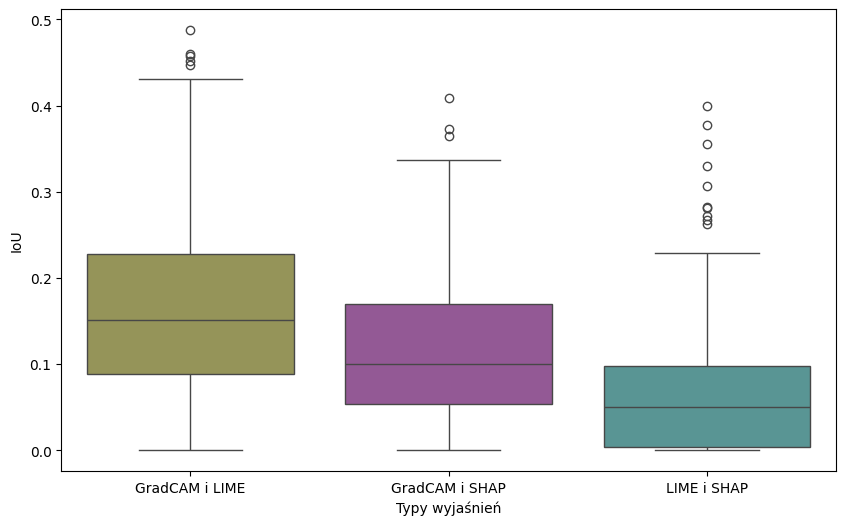
\includegraphics[width=.9\textwidth]{img/base_coherence_dog}
		\caption{\textbf{Dog}}  \label{}
	\end{subfigure}
	\begin{subfigure}[b]{0.3\textwidth}
		\centering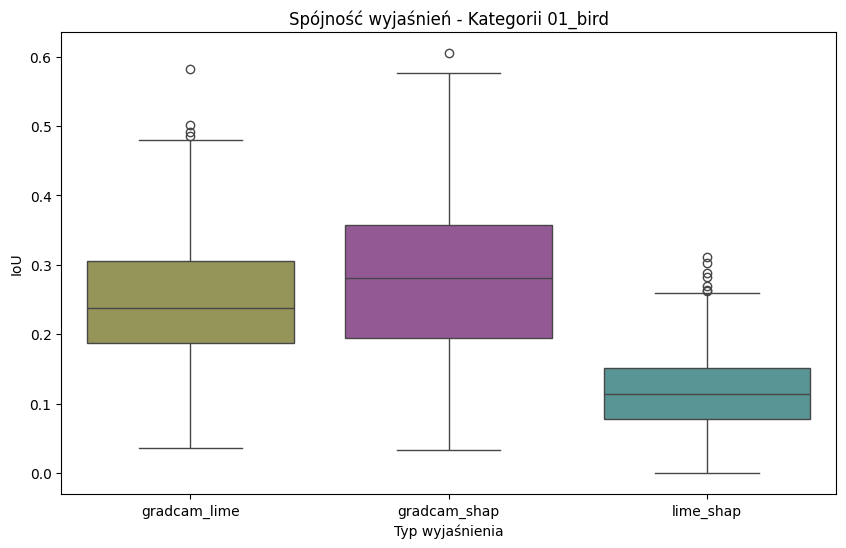
\includegraphics[width=.9\textwidth]{img/base_coherence_bird}
		\caption{\textbf{Bird}}  \label{}
	\end{subfigure}
	\begin{subfigure}[b]{0.3\textwidth}
		\centering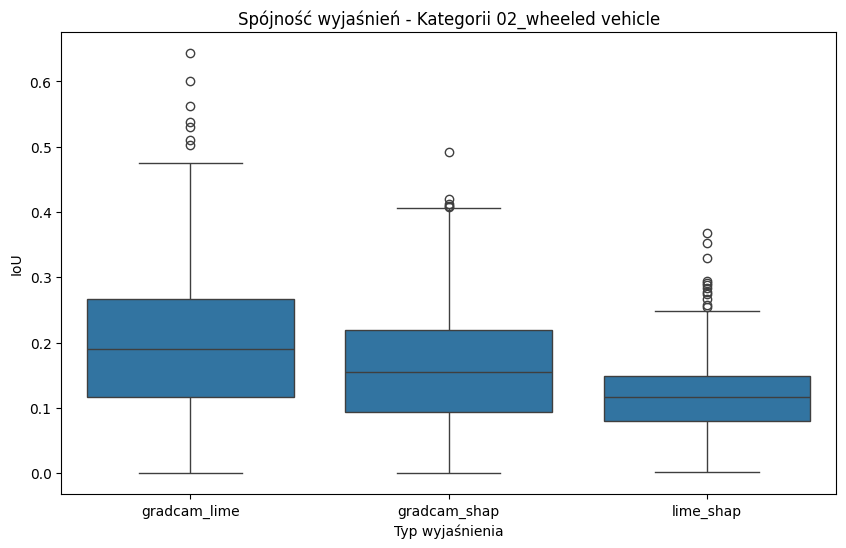
\includegraphics[width=.9\textwidth]{img/base_coherence_vehicle}
		\caption{\textbf{Vehicle}}  \label{}
	\end{subfigure}
	\begin{subfigure}[b]{0.3\textwidth}
		\centering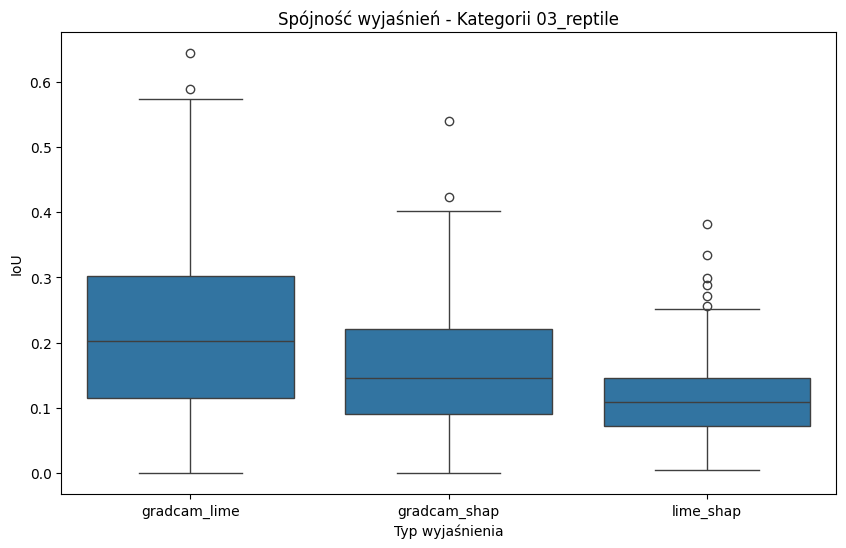
\includegraphics[width=.9\textwidth]{img/base_coherence_reptile}
		\caption{\textbf{Reptile}}  \label{}
	\end{subfigure}
	\begin{subfigure}[b]{0.3\textwidth}
		\centering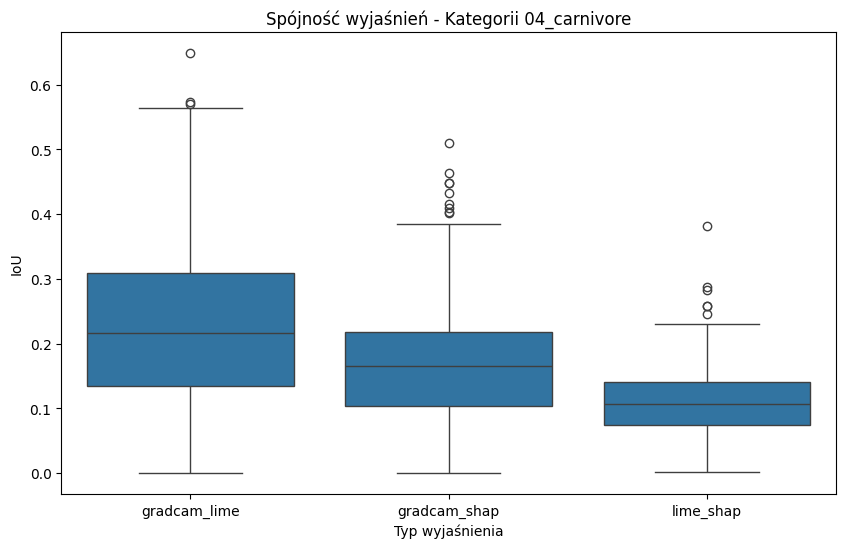
\includegraphics[width=.9\textwidth]{img/base_coherence_carnivore}
		\caption{\textbf{Carnivore}}  \label{}
	\end{subfigure}
	\begin{subfigure}[b]{0.3\textwidth}
		\centering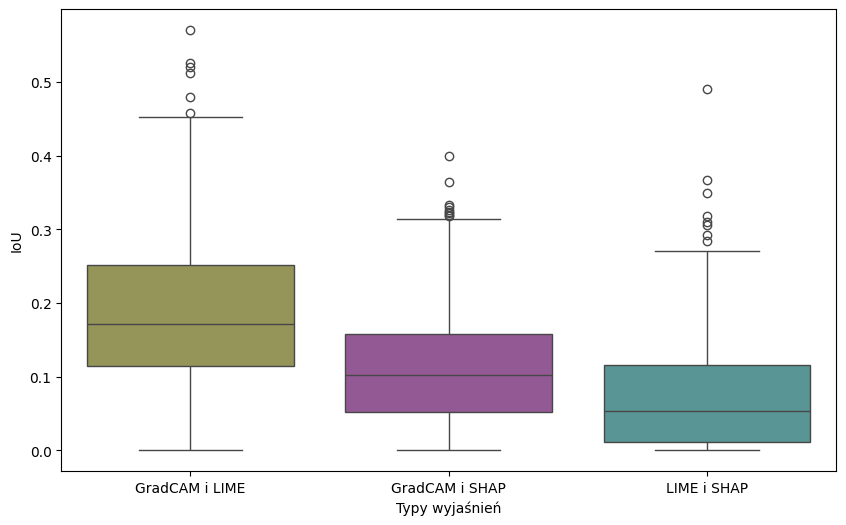
\includegraphics[width=.9\textwidth]{img/base_coherence_insect}
		\caption{\textbf{Insect}}  \label{}
	\end{subfigure}
	\begin{subfigure}[b]{0.3\textwidth}
		\centering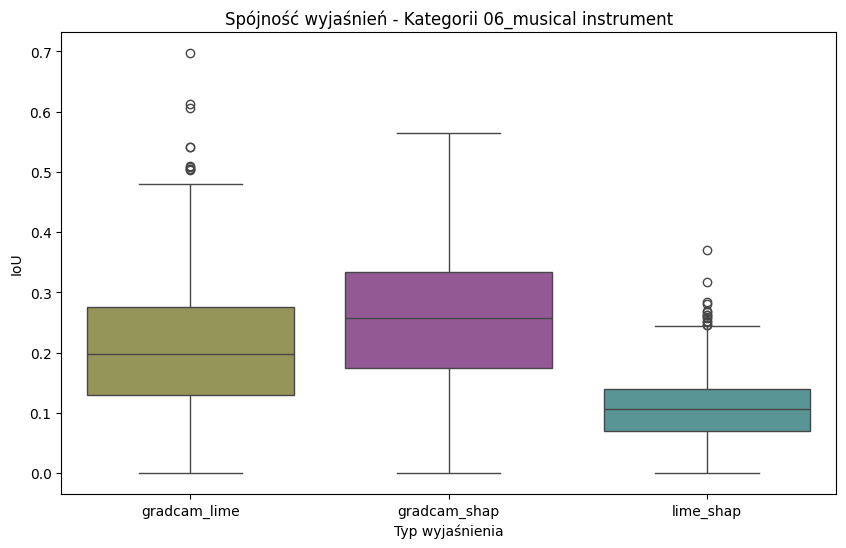
\includegraphics[width=.9\textwidth]{img/base_coherence_music}
		\caption{\textbf{Instrument}}  \label{}
	\end{subfigure}
	\begin{subfigure}[b]{0.3\textwidth}
		\centering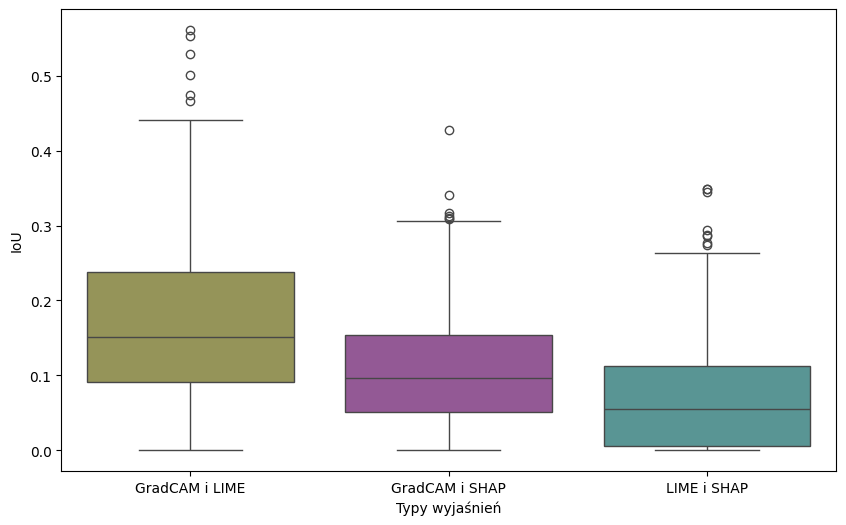
\includegraphics[width=.9\textwidth]{img/base_coherence_primate}
		\caption{\textbf{Primate}}  \label{}
	\end{subfigure}
	\begin{subfigure}[b]{0.3\textwidth}
		\centering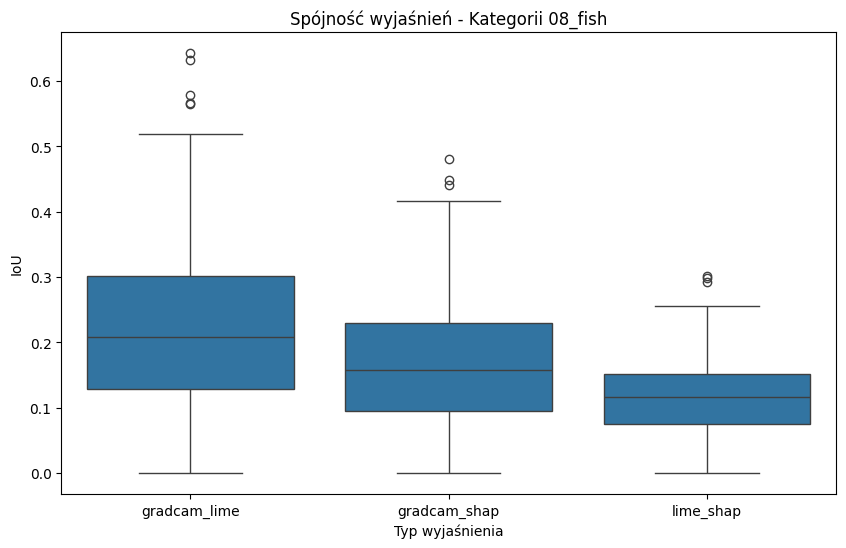
\includegraphics[width=.9\textwidth]{img/base_coherence_fish}
		\caption{\textbf{Fish}}  \label{}
	\end{subfigure}
	\caption{Spójność wyjaśnień dla różnych kategorii}
	\label{rys:coherence_category}
\end{figure}

\begin{table}[h]
	\centering
	\begin{tabular}{|c|c|c|c|}
		\hline
		\textbf{Kategoria}           & \textbf{GradCAM i LIME} & \textbf{GradCAM i SHAP} & \textbf{LIME i SHAP} \\
		\hline
		\textbf{Pies}                & 0.165114                & 0.113522                & 0.064965             \\
		\hline
		\textbf{Ptak}                & 0.165077                & 0.117948                & 0.075792             \\
		\hline
		\textbf{Pojazd na kołach}    & 0.184504                & 0.109644                & 0.070630             \\
		\hline
		\textbf{Gad}                 & 0.187232                & 0.108796                & 0.077426             \\
		\hline
		\textbf{Mięsorzerca}         & 0.167741                & 0.114880                & 0.072844             \\
		\hline
		\textbf{Insekt}              & 0.191125                & 0.112918                & 0.075120             \\
		\hline
		\textbf{Instrument muzyczny} & 0.195389                & 0.100318                & 0.073182             \\
		\hline
		\textbf{Naczelny}            & 0.169974                & 0.107942                & 0.071622             \\
		\hline
		\textbf{Ryba}                & 0.180948                & 0.113242                & 0.070721             \\
		\hline
	\end{tabular}
	\caption{Średnie wartości IoU dla różnych kategorii}
	\label{tab:base_coherence_categories}
\end{table}

Dane zostały przedstawione w ten sam sposób jak wcześniej, za pomocą wykresu (Rys \ref{rys:coherence_category}) oraz tabeli (Tabela \ref{tab:base_coherence_categories}) przedstawiającej średnie wartości IoU.

Spójności różnią się w zależności od kategorii, jednak największą spójność zawsze posiada GradCAM z LIME.
Największą spójnością dla nich są kategorie Instrument muzyczny oraz Insekt.
Najniższą spójnością natomiast dla nich są kategorie Pies i Ptak.

Najniższą spójnością cechują się zawsze LIME i SHAP, dla których najgorsze wyniki są dla kategorii Pies, natomiast najlepsze dla Gad.

GraCAM i SHAP posiadają wartości o bliskich wartościach dla wszystkich kategorii.

Kategoria Insekt jako jedyna posiada wyższą średnią IoU niż średnia IoU całego zbioru dla wszystkich typów XAI.
Natomiast kategoria Naczelny jako jedyna posiada niższą średnią IoU całego zbioru dla wszystkich typów XAI.

\vspace{1cm}
W celu zweryfikowania czy wielkość wyjaśnień miała znaczenie przeanalizowano spójność wyjaśnień podzieloną ze względu na wielkość obiektów na obrazie.

\begin{figure}[h]
	\centering
	\begin{subfigure}[b]{0.3\textwidth}
		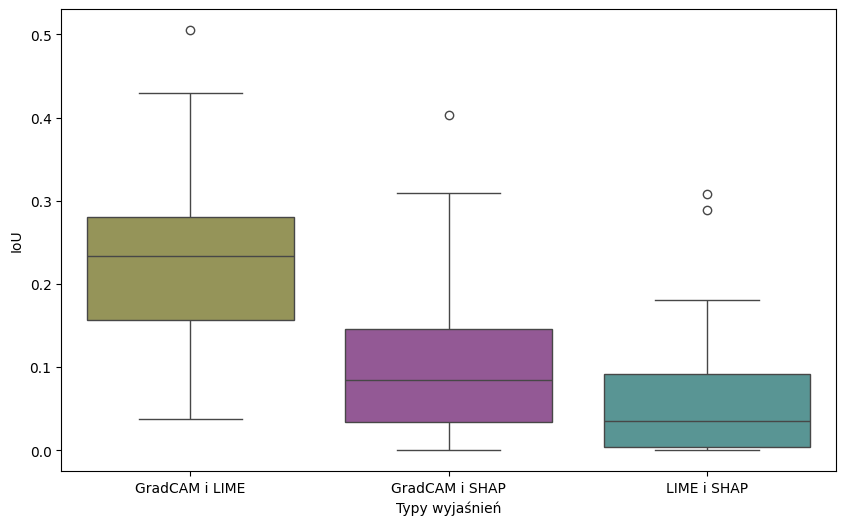
\includegraphics[width=1\textwidth]{img/base_coherence_size_XS}
		\caption{Bardzo mały obiekt}  \label{}
	\end{subfigure}
	\begin{subfigure}[b]{0.3\textwidth}
		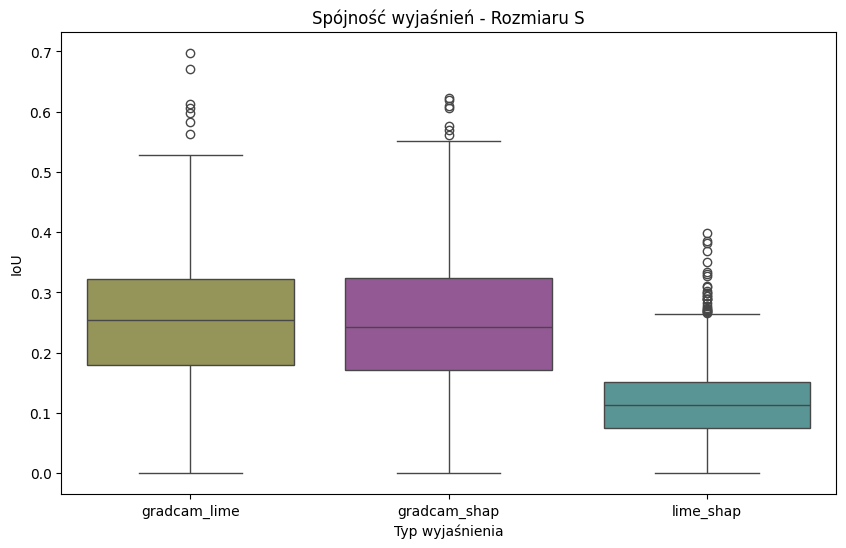
\includegraphics[width=1\textwidth]{img/base_coherence_size_S}
		\caption{Mały obiekt}  \label{}
	\end{subfigure}
	\begin{subfigure}[b]{0.3\textwidth}
		\centering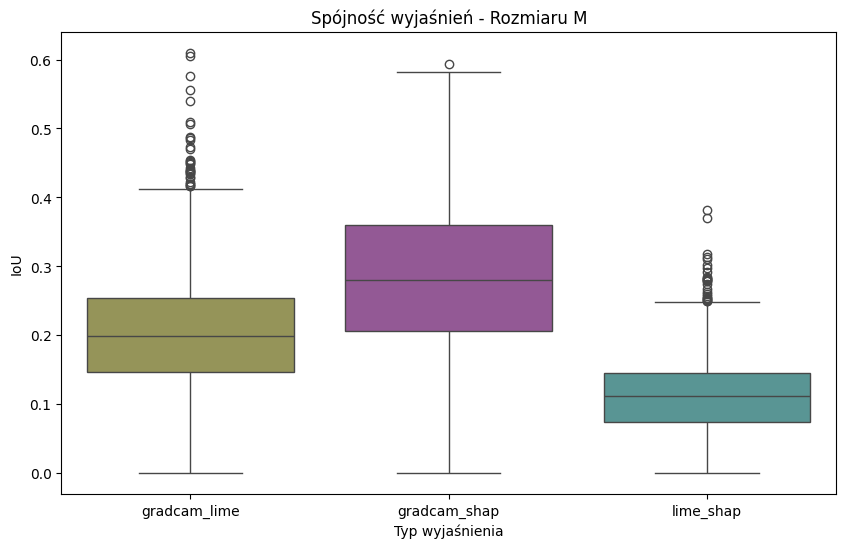
\includegraphics[width=1\textwidth]{img/base_coherence_size_M}
		\caption{Średni obiekt}  \label{}
	\end{subfigure}
	\begin{subfigure}[b]{0.3\textwidth}
		\centering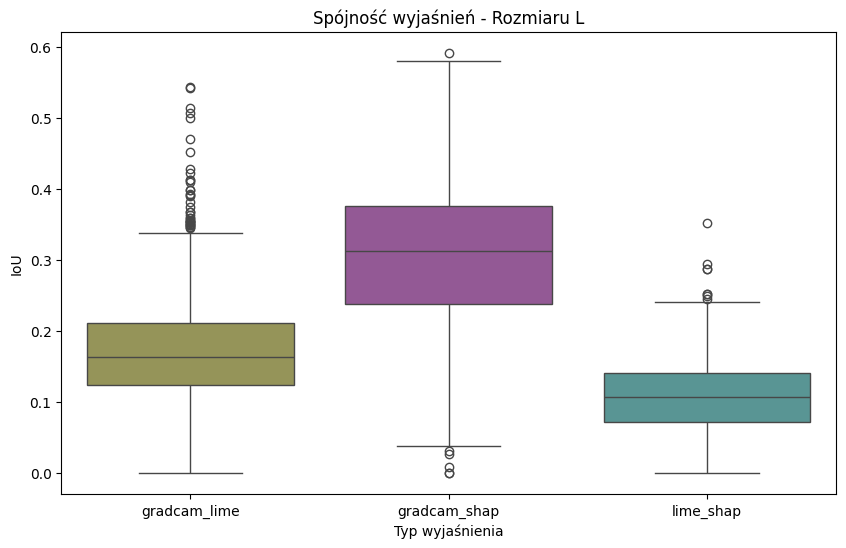
\includegraphics[width=1\textwidth]{img/base_coherence_size_L}
		\caption{Duży obiekt}  \label{}
	\end{subfigure}
	\begin{subfigure}[b]{0.3\textwidth}
		\centering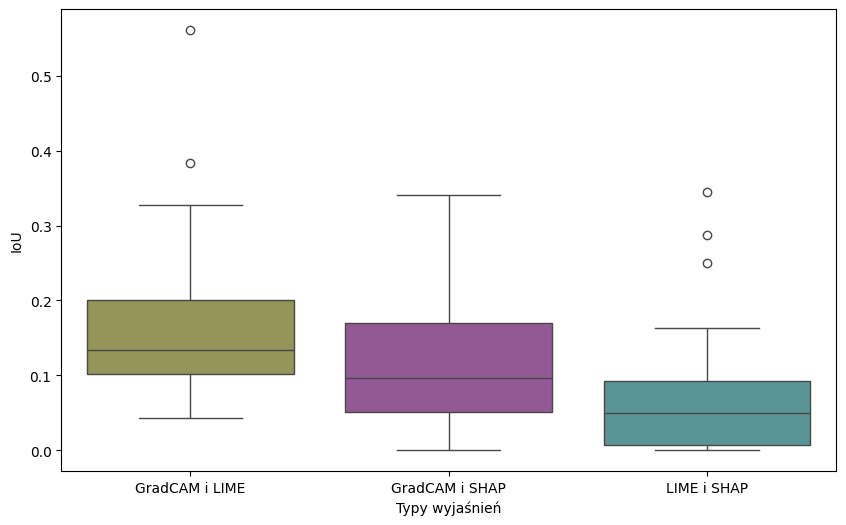
\includegraphics[width=1\textwidth]{img/base_coherence_size_XL}
		\caption{Bardzo duży obiekt}  \label{}
	\end{subfigure}
	\caption{Spójność wyjaśnień dla różnych rozmiarów obiektów}
	\label{rys:coherence_size}
\end{figure}

\begin{table}[h]
	\centering
	\begin{tabular}{|c|c|c|c|}
		\hline
		\textbf{Rozmiar}     & \textbf{GradCAM i LIME} & \textbf{GradCAM i SHAP} & \textbf{LIME i SHAP} \\
		\hline
		\textbf{Bardzo mały} & 0.230775                & 0.106354                & 0.059743             \\
		\hline
		\textbf{Mały}        & 0.191562                & 0.115253                & 0.079477             \\
		\hline
		\textbf{Średni}      & 0.175971                & 0.107933                & 0.068557             \\
		\hline
		\textbf{Duży}        & 0.166485                & 0.110300                & 0.070198             \\
		\hline
		\textbf{Bardzo duży} & 0.163015                & 0.111202                & 0.068941             \\
		\hline
	\end{tabular}
	\caption{Średnie wartości IoU dla różnych rozmiarów}
	\label{tab:base_coherence_size}
\end{table}

Tak jak w poprzednich przypadkach wyniki przedstawiono na wykresie (Rys \ref{rys:coherence_size}) oraz tabeli (Tabela \ref{tab:base_coherence_size}) przedstawiającej średnie wartości IoU dla porównania spójności wyjaśnień w zależności od rozmiaru obiektu na obrazie.

Spójności różnią się w zależności od wielkości obiektu, jednak największą spójność zawsze posiada GradCAM z LIME.
Największą spójność posiadają dla obiektów bardzo małych i ta spójność zmniejsza się wraz ze wzrostem wielkości obiektu.

GradCAM i SHAP największą spójnośc posiadają dla obiektów małych obiektów, a najmniejszą dla obiektów bardzo małych, są to jednak niewielkie różnice.

LIME i SHAP największą spójność posiadają dla obiektów małych, a najmniejszą dla obiektów bardzo małych.

